\documentclass[11pt,a4paper]{article}

% ---------------------------------------------------------------------------
% Packages
% ---------------------------------------------------------------------------
\usepackage[margin=2.5cm]{geometry}
\usepackage[utf8]{inputenc}
\usepackage[T1]{fontenc}
\usepackage{graphicx}
\usepackage{tikz}
\usetikzlibrary{shapes.geometric, arrows.meta, positioning, fit, backgrounds, calc}
\usepackage{booktabs}
\usepackage{xcolor}
\usepackage{hyperref}
\usepackage{listings}
\usepackage{enumitem}
\usepackage{caption}
\usepackage{float}
\usepackage{parskip}
\usepackage{underscore}
\usepackage[export]{adjustbox}
\usepackage{amsmath}

\hypersetup{
    colorlinks=true,
    linkcolor=blue!50!black,
    citecolor=blue!50!black,
    urlcolor=blue!50!black,
    pdftitle={Phase 3 Implementation Report -- Behavioral Preference Profile},
    pdfauthor={Narges}
}

% ---------------------------------------------------------------------------
% Color palette for diagrams (same palette as the Phase 0/1 report)
% ---------------------------------------------------------------------------
\definecolor{dbcolor}{RGB}{215,235,250}
\definecolor{actualcolor}{RGB}{225,245,225}
\definecolor{statedcolor}{RGB}{255,235,205}
\definecolor{pipelinecolor}{RGB}{240,225,245}
\definecolor{outcolor}{RGB}{255,225,225}
\definecolor{boxborder}{RGB}{80,80,80}

\tikzset{
    block/.style={rectangle, draw=boxborder, rounded corners, thick,
        text width=3.2cm, minimum height=1.1cm, align=center, font=\small},
    smallblock/.style={rectangle, draw=boxborder, rounded corners, thick,
        text width=2.6cm, minimum height=0.9cm, align=center, font=\footnotesize},
    arrow/.style={-{Latex[length=2.5mm]}, thick}
}

% ---------------------------------------------------------------------------
% Listings style
% ---------------------------------------------------------------------------
\lstset{
    basicstyle=\ttfamily\footnotesize,
    breaklines=true,
    frame=single,
    backgroundcolor=\color{gray!7},
    columns=fullflexible,
    showstringspaces=false,
    xleftmargin=1em,
    xrightmargin=1em,
    aboveskip=8pt,
    belowskip=8pt
}

\newcommand{\code}[1]{\texttt{#1}}

\title{\Large \textbf{A Query Recommender for Preference-Aware Natural Language Querying} \\[4pt]
\large Implementation Report --- Phase 3 (Behavioral Preference Profile) \\[2pt]
\normalsize \emph{The ``stated vs.\ actual preference'' signal for the query recommender}}
\author{Narges \\ \small Supervisor: Prof. Elisa Quintarelli}
\date{\today}

\begin{document}

\maketitle

\begin{abstract}
\noindent
This report documents Phase 3 of the thesis: the construction of a per-user \textbf{behavioral
preference profile} on the Movie domain, contrasting what a user \emph{says} they want (inferred
from free-text search queries) against what they \emph{actually} engage with (inferred from
weighted watch behavior). This is the empirical substrate for the thesis's central premise ---
that stated and real preferences diverge, and that a query recommender must condition on both to
be useful. Unlike Phase 0/1 (data/infrastructure preparation and a development harness, reported
separately and not thesis deliverables in their own right), Phase 3 \textbf{is} part of the
thesis's actual contribution: it produces the behavioral divergence signal that Phase 4's
candidate-generation step will consume. This report first gives a high-level overview of the
pipeline that produces this signal, then explains each part of it in detail, and reports the
verification results obtained on the full \code{netflix\_dataset}.
\end{abstract}

\tableofcontents
\newpage

% =============================================================================
\section{Introduction}
% =============================================================================

The professor's scoping email attributes to ``Jerry's'' analysis the observation that a user's
\emph{stated} queries and their \emph{real} interaction behavior often diverge --- a user may
type \emph{``romantic movie''} but consistently watch American comedies. A query recommender that
only looks at query history is, per this framing, little more than autocomplete; a genuinely
useful one must condition on both signals. Phase 3 builds the first half of that requirement: a
machine-readable, per-user summary of what a user says they want versus what they actually engage
with, quantified as a single divergence score.

\subsection{Scope}

Phase 3 operates on the \textbf{Movie domain only}. As established during Phase 0, the Tourism
domain's only large behavioral table (\code{log\_vc}, VeronaCard tap-in visits) is keyed to an
anonymous card, not a named user, and was explicitly excluded from the ontology --- so Tourism has
no per-user behavioral signal to condition on. All behavior-aware work in this thesis is
therefore carried by the Movie domain's \code{netflix\_dataset/} (a synthetic, Faker-generated
dataset with 10{,}300 users, 1{,}040 movies, 105{,}000 watch events, and 26{,}500 search-log
entries).

\subsection{Where this fits}

Phase 3 is implemented as a standalone script, \code{recommender/behavioral\_profile.py}, in a
new top-level \code{recommender/} directory --- the start of the actual thesis deliverable,
per the scope decision recorded in the companion \emph{Phase 0 \& Phase 1 Implementation Report}.
It is kept separate from \code{profile\_geneartion/} (an earlier, more general interest-profile
tool from the system's original architecture), which remains a reference for the interest-node
JSON shape but is not extended in place. Phase 3's output --- one JSON profile per user --- is the
direct input to Phase 4's recommendation-candidate generation step, described in the project
roadmap.

\newpage
% =============================================================================
\section{High-Level Overview}
% =============================================================================

\subsection{The core idea}

For each user, Phase 3 computes two independent rankings over the same vocabulary of catalog
categories (genre, content type, country of origin): one derived from what they \emph{searched
for}, one from what they \emph{watched}. It then measures how much the two rankings agree. Three
design choices make this measurement meaningful rather than a raw count comparison:

\begin{enumerate}[label=(\alph*)]
    \item \textbf{Weighting, not counting.} A watch event that a user completed counts more than
        one they abandoned after 5\%; this is implemented as a continuous \emph{completion
        weight} rather than a binary ``watched / not watched'' signal (Section~\ref{sec:actual}).
    \item \textbf{An engineered link between the two data sources.} \code{search\_logs} and
        \code{watch\_history} share no foreign key in the source dataset --- there is no column
        recording which movie, if any, a search led to. A temporal join (nearest subsequent watch
        within a time window) is engineered to recover this link where it plausibly exists
        (Section~\ref{sec:link}), producing a concrete artifact of individual
        search$\to$watch events, independent of the aggregate divergence score.
    \item \textbf{A single summary statistic.} The two rankings' top-5 categories are compared via
        Jaccard similarity, giving one number per user that later phases (and this report's
        results) can reason about directly (Section~\ref{sec:divergence}).
\end{enumerate}

\subsection{Pipeline diagram}

Figure~\ref{fig:overview} shows the full data flow, from the three source CSVs to the two output
artifacts. The left branch (green) computes the \emph{actual} signal from watch behavior; the
right branch (orange) computes the \emph{stated} signal from search behavior. Both converge on a
per-user divergence score and a combined JSON profile.

\begin{figure}[H]
\centering
\begin{adjustbox}{max width=\textwidth, max totalheight=0.9\textheight, center}
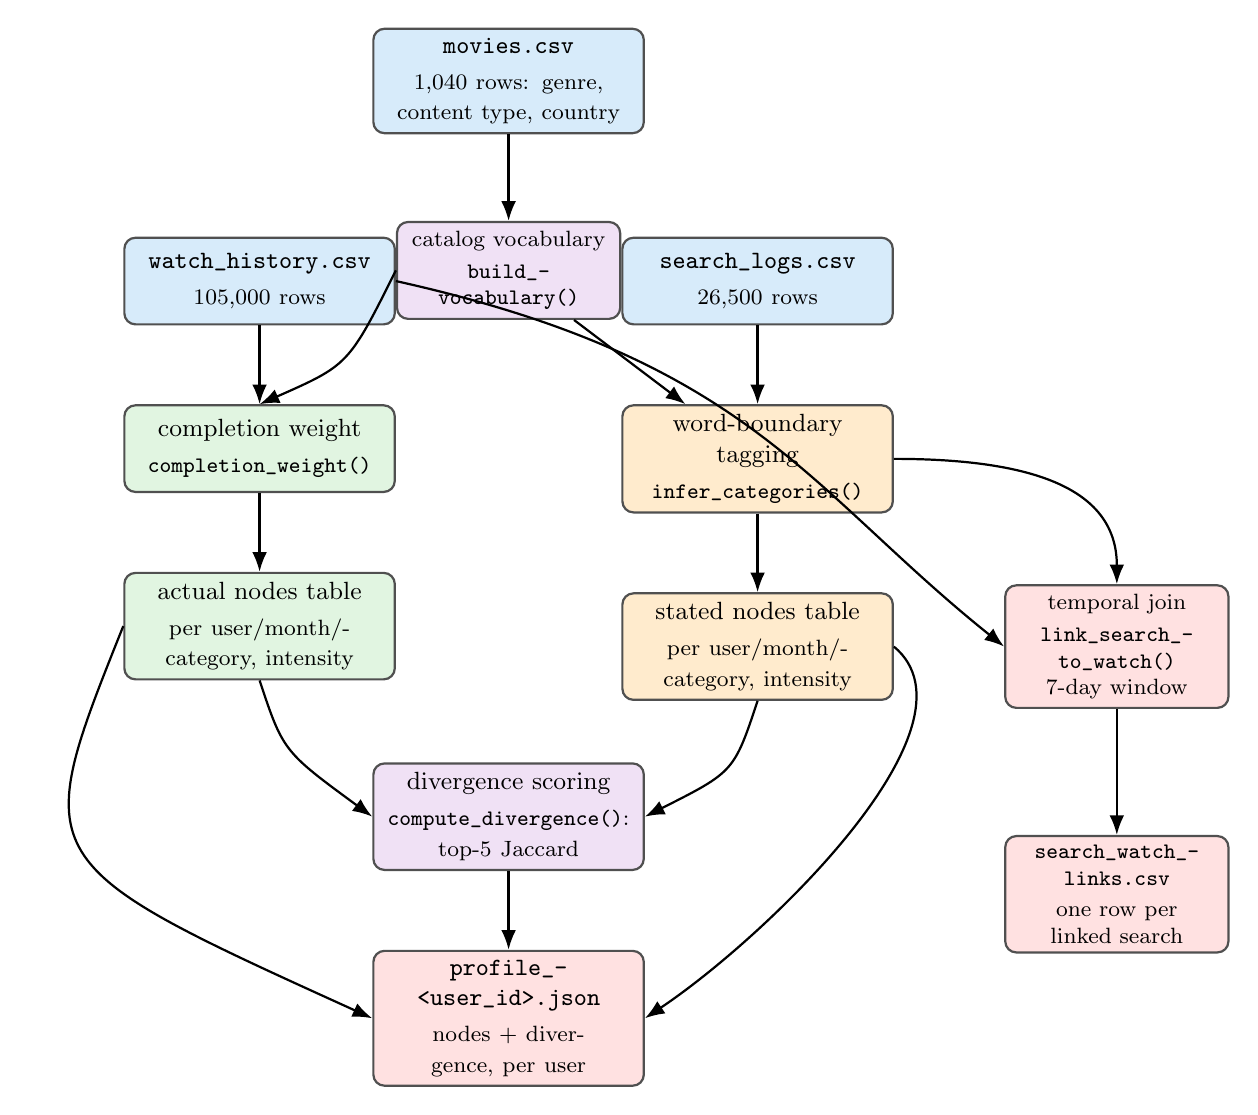
\begin{tikzpicture}[node distance=1.0cm and 1.3cm]

    \node[block, fill=dbcolor] (movies) {\code{movies.csv}\\[2pt]\footnotesize 1{,}040 rows: genre, content type, country};
    \node[block, fill=dbcolor, below left=1.3cm and -0.3cm of movies] (watch) {\code{watch\_history.csv}\\[2pt]\footnotesize 105{,}000 rows};
    \node[block, fill=dbcolor, below right=1.3cm and -0.3cm of movies] (search) {\code{search\_logs.csv}\\[2pt]\footnotesize 26{,}500 rows};

    \node[smallblock, fill=pipelinecolor, below=1.1cm of movies] (vocab) {catalog vocabulary\\[2pt]\footnotesize \code{build\_vocabulary()}};

    \node[block, fill=actualcolor, below=of watch] (weight) {completion weight\\[2pt]\footnotesize \code{completion\_weight()}};
    \node[block, fill=statedcolor, below=of search] (tag) {word-boundary tagging\\[2pt]\footnotesize \code{infer\_categories()}};

    \node[block, fill=actualcolor, below=of weight] (actualtab) {actual nodes table\\[2pt]\footnotesize per user/month/category, intensity};
    \node[block, fill=statedcolor, below=of tag] (statedtab) {stated nodes table\\[2pt]\footnotesize per user/month/category, intensity};

    \node[smallblock, fill=outcolor, right=1.4cm of statedtab] (link) {temporal join\\[2pt]\footnotesize \code{link\_search\_to\_watch()}\\ 7-day window};

    \coordinate (midAS) at ($(actualtab)!0.5!(statedtab)$);
    \node[block, fill=pipelinecolor, below=1.6cm of midAS] (div) {divergence scoring\\[2pt]\footnotesize \code{compute\_divergence()}: top-5 Jaccard};

    \node[block, fill=outcolor, below=of div] (out) {\code{profile\_<user\_id>.json}\\[2pt]\footnotesize nodes + divergence, per user};
    \node[smallblock, fill=outcolor, below=1.6cm of link] (links) {\code{search\_watch\_links.csv}\\[2pt]\footnotesize one row per linked search};

    \draw[arrow] (movies) -- (vocab);
    \draw[arrow] (vocab) -- (tag);
    \draw[arrow] (vocab.west) .. controls +(-0.6,-1.2) .. (weight.north);
    \draw[arrow] (watch) -- (weight);
    \draw[arrow] (search) -- (tag);
    \draw[arrow] (weight) -- (actualtab);
    \draw[arrow] (tag) -- (statedtab);
    \draw[arrow] (tag.east) .. controls +(1.8,0) and +(0,1.2) .. (link.north);
    \draw[arrow] (watch.east) .. controls +(4.5,-1.0) and +(-2.5,2.0) .. (link.west);
    \draw[arrow] (actualtab.south) .. controls +(0.3,-0.9) .. (div.west);
    \draw[arrow] (statedtab.south) .. controls +(-0.3,-0.9) .. (div.east);
    \draw[arrow] (div) -- (out);
    \draw[arrow] (actualtab.west) .. controls +(-1.2,-3.0) .. (out.west);
    \draw[arrow] (statedtab.east) .. controls +(1.2,-1.0) and +(1.5,1.0) .. (out.east);
    \draw[arrow] (link) -- (links);

\end{tikzpicture}
\end{adjustbox}
\caption{Phase 3 data flow. The catalog vocabulary (top) is used both to tag search queries and,
implicitly, to define the category space watch events are grouped into. The actual (green) and
stated (orange) branches each produce a per-user/month/category intensity table; these feed both
the per-user JSON profiles (with all nodes plus a divergence summary) and, independently, a
divergence score. The temporal join (bottom left, red) produces a separate, row-level output.}
\label{fig:overview}
\end{figure}

\newpage
% =============================================================================
\section{Detailed Walkthrough}
% =============================================================================

This section explains each stage of \code{recommender/behavioral\_profile.py} (244 lines) in the
order it executes, from \code{main()}.

\subsection{Inputs}

\code{load\_data()} reads the three source CSVs and left-joins \code{watch\_history} against
\code{movies} on \code{movie\_id} to attach each watch event's genre/content-type/country. Rows
with a missing \code{user\_id} or \code{movie\_id} are dropped. Missing category values in the
catalog are filled with the literal string \code{"Unknown"} so downstream groupings do not
silently drop rows with incomplete metadata.

\subsection{Catalog vocabulary and search-query tagging}
\label{sec:vocab}

\code{build\_vocabulary()} collects every distinct, non-``Unknown'' value across
\code{genre\_primary}, \code{genre\_secondary}, \code{content\_type}, and
\code{country\_of\_origin}, sorted \textbf{longest string first}. This ordering matters: it
guarantees a multi-word value such as \code{"Stand-up Comedy"} is checked before a shorter value
like \code{"Comedy"} could match part of it.

\code{infer\_categories()} then tags each free-text \code{search\_query} with every vocabulary
value it contains, using a \textbf{word-boundary regular expression} (\verb|\bvalue\b|), not a
plain substring test. This is a deliberate bug fix made during implementation:

\begin{lstlisting}[language=Python, caption={The word-boundary tagging function. An earlier,
substring-based version let \code{content\_type="Movie"} match inside the plural word ``movies''
in nearly every query, and would similarly have let \code{"War"} match inside ``warrior.''}]
def build_vocabulary_patterns(vocabulary):
    # word-boundary match: plain substring would let e.g. "Movie" (a content_type
    # value) spuriously match inside the plural "movies", or "War" match inside
    # "warrior"
    return {v: re.compile(r"\b" + re.escape(v.lower()) + r"\b") for v in vocabulary}

def infer_categories(search_query, vocabulary_patterns):
    query = str(search_query).lower()
    return [v for v, pattern in vocabulary_patterns.items() if pattern.search(query)]
\end{lstlisting}

\subsection{Actual-interest weighting}
\label{sec:actual}

\code{completion\_weight()} converts each \code{watch\_history} row into a weight in
$[0.05, 1.0]$:

\[
w(\text{row}) =
\begin{cases}
1.0 & \text{if } \code{action} = \code{"completed"} \\[4pt]
\operatorname{clip}\!\left(\dfrac{\code{progress\_percentage}}{100},\, 0.05,\, 1.0\right) &
    \text{if progress is known} \\[8pt]
0.3 & \text{otherwise}
\end{cases}
\]

This operationalizes ``actual interest'' as \emph{how much} of something a user engaged with, not
merely whether a watch event was logged --- a user who starts and abandons five thrillers should
not count for as much as one who finishes a single thriller.

\code{compute\_actual\_nodes\_table()} groups weighted watches by
\code{(user\_id, month, category-value)}, divides by that user-month's total weighted
interactions to obtain a relative \textbf{intensity} in $[0,1]$ (rounded to two decimals, the
same relative-share convention used by the earlier \code{profile\_geneartion} interest-node
model), and labels every row \code{signal = "actual"}.

\subsection{Search{\textrightarrow}watch temporal join}
\label{sec:link}

\code{link\_search\_to\_watch()} addresses a gap identified during data inventory: there is no
existing key linking a \code{search\_logs} row to a specific movie in \code{watch\_history}. For
every search with at least one inferred category (Section~\ref{sec:vocab}), the function finds
that user's \textbf{next watch within a 7-day window}, implemented with \code{pandas}'
\code{merge\_asof} (forward direction, 7-day tolerance, grouped \code{by="user\_id"}):

\begin{lstlisting}[language=Python, caption={The temporal join. \code{matched\_stated\_intent}
flags whether any category inferred from the search actually appears among the linked watch's
own genre/content-type --- a row-level, individually inspectable artifact of stated-vs-actual
correspondence, independent of the aggregate divergence score in Section~\ref{sec:divergence}.}]
linked = pd.merge_asof(
    searches, watch_sorted,
    left_on="search_date", right_on="watch_date", by="user_id",
    direction="forward", tolerance=pd.Timedelta(days=7),
    suffixes=("", "_watched"),
)
linked = linked.dropna(subset=["movie_id"]).copy()
linked["matched_stated_intent"] = linked.apply(
    lambda r: bool(set(r["inferred_categories"])
                   & {r["genre_primary"], r["genre_secondary"], r["content_type"]}),
    axis=1,
)
\end{lstlisting}

Rows without a watch inside the window are dropped, so the resulting table (written to
\code{search\_watch\_links.csv}) contains only searches that were plausibly followed by a
corresponding viewing session.

\subsection{Stated-interest weighting}

\code{compute\_stated\_nodes\_table()} mirrors Section~\ref{sec:actual}'s computation for the
stated side: each search's inferred categories are exploded into one row per category, grouped by
\code{(user\_id, month, category)}, and normalized by that user-month's total tagged-search count
to give an intensity in $[0,1]$. Rows are labeled \code{signal = "stated"}.

\subsection{Divergence scoring}
\label{sec:divergence}

\code{compute\_divergence()} takes each user's \textbf{top-5} actual categories and top-5 stated
categories, ranked by summed intensity across all months, and computes:

\begin{itemize}
    \item \code{overlap} --- the set intersection of the two top-5 lists;
    \item \code{jaccard\_similarity} --- $|A \cap S| / |A \cup S|$ for actual set $A$ and stated
        set $S$ (\code{None} if a user has neither signal at all).
\end{itemize}

This single number is the behavioral divergence signal Phase 4's candidate generation and ranking
will condition on.

\subsection{Output writing}

\code{write\_user\_profiles()} concatenates the actual and stated node tables, groups by
\code{user\_id}, and writes one JSON file per user to
\code{recommender/output/behavioral\_profiles/profile\_<user\_id>.json}, combining every node
(actual and stated, across all months) with that user's single divergence summary. The full
schema is given in Section~\ref{sec:schema}.

\newpage
% =============================================================================
\section{Output Schema}
\label{sec:schema}
% =============================================================================

\begin{lstlisting}[language=, caption={\code{profile\_<user\_id>.json} schema.}]
{
  "user_id": "user_00001",
  "domain": "Movie",
  "nodes": [
    {
      "category": "Genre | Content Type | Country | Stated Interest",
      "value": "<category value>",
      "signal": "actual | stated",
      "intensity": 0.0-1.0,
      "time_window": { "type": "monthly", "value": "YYYY-MM" },
      "support": { "weighted_interactions": <float> }
                 | { "searches": <int> }
    }
  ],
  "divergence": {
    "actual_top": ["<top-5 actual categories by intensity>"],
    "stated_top": ["<top-5 stated categories by intensity>"],
    "overlap": ["<categories in both>"],
    "jaccard_similarity": 0.0-1.0
  }
}
\end{lstlisting}

This is structurally analogous to the earlier \code{profile\_geneartion} tool's
\code{nodi\_interesse} shape (the same category/value/intensity/time-window fields), extended
with the \code{signal} field distinguishing stated from actual, and the top-level
\code{divergence} block summarizing the gap between them.

% =============================================================================
\section{Verification and Results}
% =============================================================================

The script was run against the full \code{netflix\_dataset} (1{,}040 movies, 10{,}300 users,
105{,}000 watch rows, 26{,}500 search rows).

\begin{table}[H]
\centering
\begin{tabular}{lr}
\toprule
\textbf{Metric} & \textbf{Value} \\
\midrule
Users with a behavioral profile written & 10{,}000 of 10{,}300 \\
Search$\to$watch links found (7-day window) & 1{,}179 \\
Average stated-vs-actual Jaccard similarity & \textbf{0.01} \\
Users with zero overlap (top-5 stated vs.\ top-5 actual) & \textbf{9{,}399 / 10{,}000} \\
\bottomrule
\end{tabular}
\caption{Phase 3 verification results on the full dataset. 300 users have no watch history and
therefore receive no profile.}
\label{tab:phase3-results}
\end{table}

As a spot check, \code{profile\_user\_00001.json} was inspected directly: its actual top-5 was
\code{["Movie", "USA", "Canada", "Adventure", "War"]} (a mix of content-type, country, and genre
values, since all three category types share one ranking pool), its stated top-5 was
\code{["Action"]} (this user had only one tagged search in the log), the overlap was empty, and
the Jaccard similarity was \code{0.0} --- consistent with the aggregate numbers above.

The word-boundary fix (Section~\ref{sec:vocab}) was confirmed to be working: searches containing
the plural word ``movies'' no longer spuriously tag \code{content\_type="Movie"}, and
``warrior''-type queries no longer spuriously tag \code{genre="War"}.

% =============================================================================
\section{Interpretation and Limitations}
% =============================================================================

\begin{itemize}
    \item \textbf{The near-zero average Jaccard similarity (0.01) is a striking number}, and its
        \emph{direction} is consistent with the professor's own framing example (a user types
        ``romantic movie'' but consistently watches American comedies). It should \textbf{not},
        however, be reported as a validated real-world divergence rate. \code{netflix\_dataset} is
        Faker-generated synthetic data with \textbf{no true causal link} between a search string
        and a later watch event --- a search and a subsequent watch being uncorrelated is exactly
        what random generation would produce, so this number reflects the heuristic's behavior on
        synthetic data at least as much as it reflects a real ``stated $\neq$ actual''
        phenomenon. This caveat must be stated explicitly in the thesis text, not presented as an
        empirical finding about real users.
    \item \textbf{The 7-day linking window is a heuristic choice}, not derived from the data. A
        different window would change the link count and, likely, the divergence number. A
        sensitivity check (e.g.\ re-running at 3, 14, and 30 days) is worth doing if this number
        is used quantitatively rather than only descriptively in the thesis.
    \item \textbf{Not yet incorporated}: recency weighting (older watches currently count equally
        with recent ones) and \code{reviews.csv} sentiment as a third signal. Both are left for a
        later iteration if the divergence signal needs refining for Phase 4.
    \item \textbf{Worth re-running once real interaction data becomes available} (e.g.\ from the
        bachelor students' external application) as a real-world comparison point against this
        synthetic-data baseline.
\end{itemize}

% =============================================================================
\section{Summary and Next Steps}
% =============================================================================

Phase 3 delivers a verified, per-user behavioral divergence signal on the Movie domain: 10{,}000
JSON profiles, each pairing a stated-interest ranking with an actual-interest ranking and a
single Jaccard divergence score, plus a row-level search$\to$watch link table. This is the first
concrete piece of the thesis's actual contribution (as opposed to the Phase 0/1 harness it is
built on top of, documented separately).

\textbf{Phase 4}, not yet built, is the direct consumer of this output: candidate query
generation will retrieve a user's semantically similar past queries (embedding-based retrieval
over their query log), combine them with a compact rendering of this phase's
\code{divergence} block in an LLM prompt (following the GQR/RA-GQR generation pattern from the
literature review), validate candidates against the currently loaded domain schema, rank them
along a query-similarity vs.\ behavior-similarity axis, and expose the result as a
\code{POST /recommend} API endpoint returning three suggested queries. Full detail on Phase 4
onward is tracked in the project roadmap document, \emph{Thesis Project Plan}.

\end{document}
